\documentclass[./\jobname.tex]{subfiles}
\begin{document}
%
\chapter{Up / Down Counter}
%
\section{Einleitung}
%
In der zweiten Aufgabe soll ein n-Bit Up / Down Counter implementiert werden. Folgende Anforderungen werden an den Up / Down Counter gestellt:
%
\begin{itemize}
	\item synchrone Logik \pfeil \enquote{clk50m} ist die Clock aller Flipflops.
	\item Aktiver Low-Reset auf Null (\enquote{rst\_n}).
	\item Zähler wird inkrementiert oder dekrementiert, wenn en == 1'b1.
	\begin{itemize}
		\item If (down == 1'b1) \pfeil\( cnt = cnt-1\)
		\item sonst \pfeil \(cnt = cnt + 1\)
	\end{itemize}
\end{itemize}
%
Zusätzlich zu den Anforderungen muss die Implementierung getestet und verifiziert werden. Dies bedeutet, dass alle Eingänge stimuliert und alle Signale im \enquote{Wave Window} angezeigt werden.
%
\section{Implementierung}
%
Die Implementierung erfolgt wie in \autoref{lst:counter_updn} dargestellt ist. In Codezeile \cref{code: parameter width} wird der Ausgang Counter \enquote{cnt} mit variabler Bitlänge definiert definiert.
%
\lstinputlisting[language=Verilog,label={lst:counter_updn}, caption=Implementierung]{./../code/counter_updn/src/counter_updn.sv}
%
\section{Test Bench}
%
In \autoref{lst:tb_counter_updn} ist die Testbench ersichtlich. Es wurde ein automatisiertes Testscript erstellt, welches einen Fehler ausgibt, sobald der Up oder Down Test fehlschlägt (Codezeile \ref{code: countUp testA} bis \ref{code: countUp testB} und \ref{code: countDown testA} bis \ref{code: countDown testB}). 
%
\lstinputlisting[language=Verilog,label={lst:tb_counter_updn}, caption=Testbench für den Up / Down Counter]{./../code/counter_updn/sim/tb_counter_updn.sv}
%
\section{Simulationsscript}
%
In \autoref{lst:sim_tb_counter_updn} ist das Simulationsscript dargestellt. Es beinhaltet dieselben Befehle wie in der letzten Lehrveranstaltung, natürlich angepasst an den Up / Down Counter.
%
\lstinputlisting[language=tcl,label={lst:sim_tb_counter_updn}, caption=Simulationsscript]{./../code/counter_updn/sim/sim_tb_counter_updn.tcl}
%
\section{Transkript und Waveform Window}
%
In \autoref{fig: wavewindow_up_down} ist das Waveform Window dargestellt. Es zeigt die geforderten Testfälle. Wie zu sehen ist, wurden die Anforderungen erfüllt.
%
\begin{figure}[H]
	\centering
	\noindent\adjustbox{max width=\textwidth}{%falls größer als \textwidth, wird das Bild verkleinert
		%trim option's parameter order: left bottom right top
		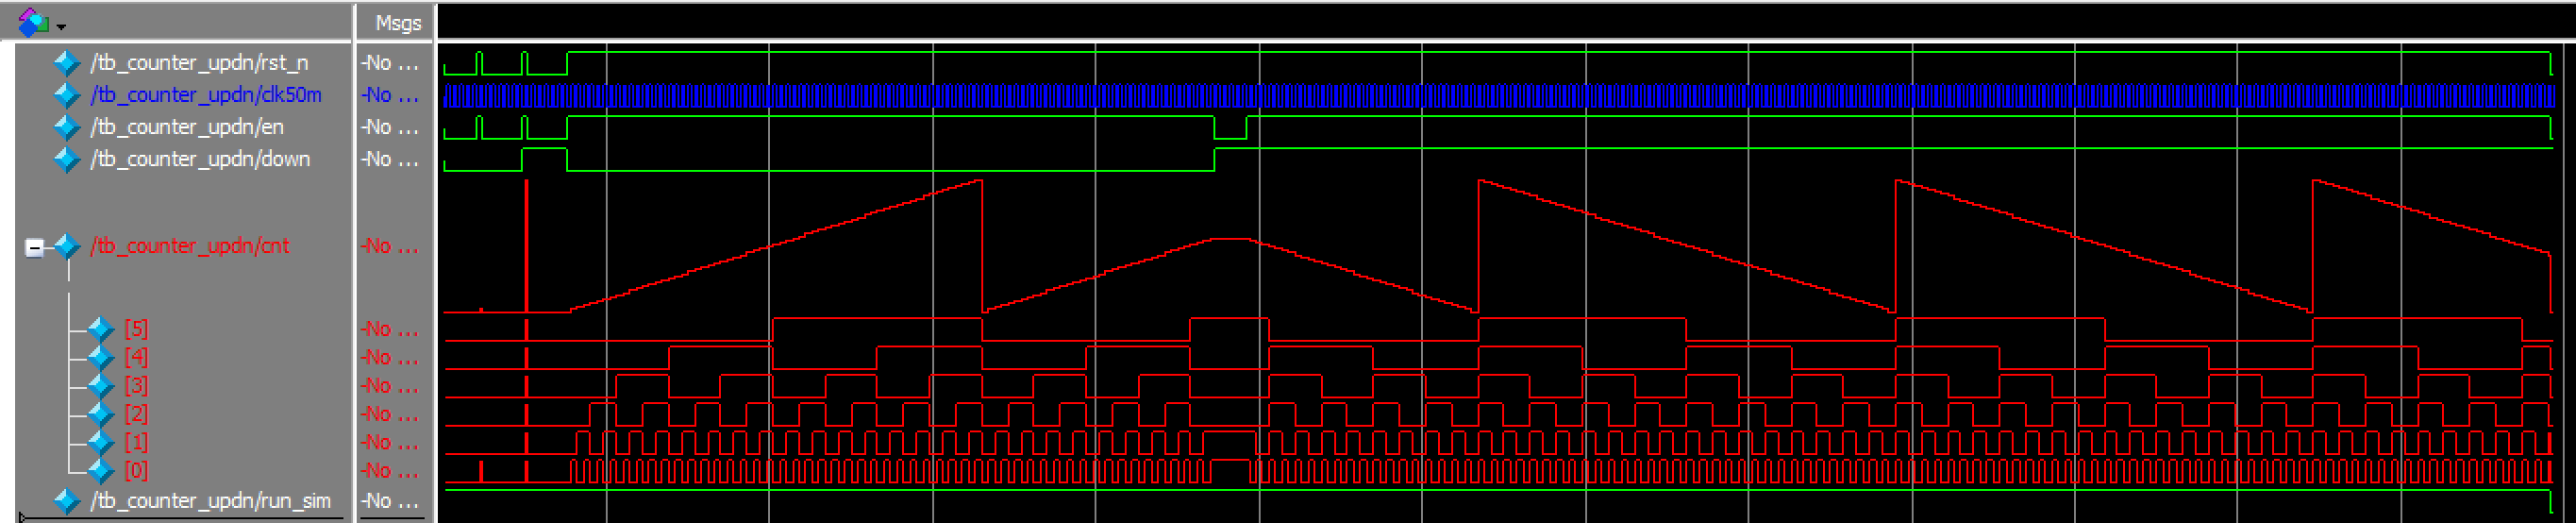
\includegraphics[width=1\textwidth]{./../code/counter_updn/doc/wavewindow_up_down.PNG}
	}
	\unterschrift{Waveform Window}{eigene Ausarbeitung}{}
	\label{fig: wavewindow_up_down}
\end{figure}
%
In \autoref{ausgabeTwo} ist der Output des Testcripts zu sehen. Alle Testfälle wurden bestanden.
%
\lstinputlisting[language=tcl,
label={ausgabeTwo}, caption=Commandline Output A]{./../code/counter_updn/doc/console_output.txt}
%
\section{Vor- und Nachteile der Implementierung}
%
Folgend sind die Vor- und Nachteile der Implementierung gelistet:
%
\begin{description}
	\item[Vorteile] \hfil
	\begin{itemize}
		\item Variable Bitlänge
	\end{itemize}
	\item[Nachteile] \hfil
	\begin{itemize}
		\item Die Clock Frequenz darf nur so hoch gewählt werden, wie es das \enquote{Back Propagation Delay} erlaubt. Somit ist die maximale Zählfrequenz begrenzt.
		\item Bei Anwahl des Down-Bits sollte beim Reseten der Counter Wert nicht auf \enquote{0} initalisiert werden, sondern mit dem maximalen Wert
		\begin{align}
		2~<<~ (`counterSize-1) - 1
		\end{align}
		\item Ebenfalls wäre es gut, den Startwert des Counters selbst wählen zu können.
	\end{itemize}
\end{description}
%
\end{document}
